\documentclass[10pt,letterpaper]{article}
\usepackage{graphicx}
\usepackage[margin=.2in]{geometry} % Adjusts the page margins.
\usepackage{setspace}             % For controlling line spacing.

\begin{document}
\pagestyle{empty} % Removes page numbers.
\setstretch{0.9}  % Reduces line spacing a bit to fit the content.

\begin{center}
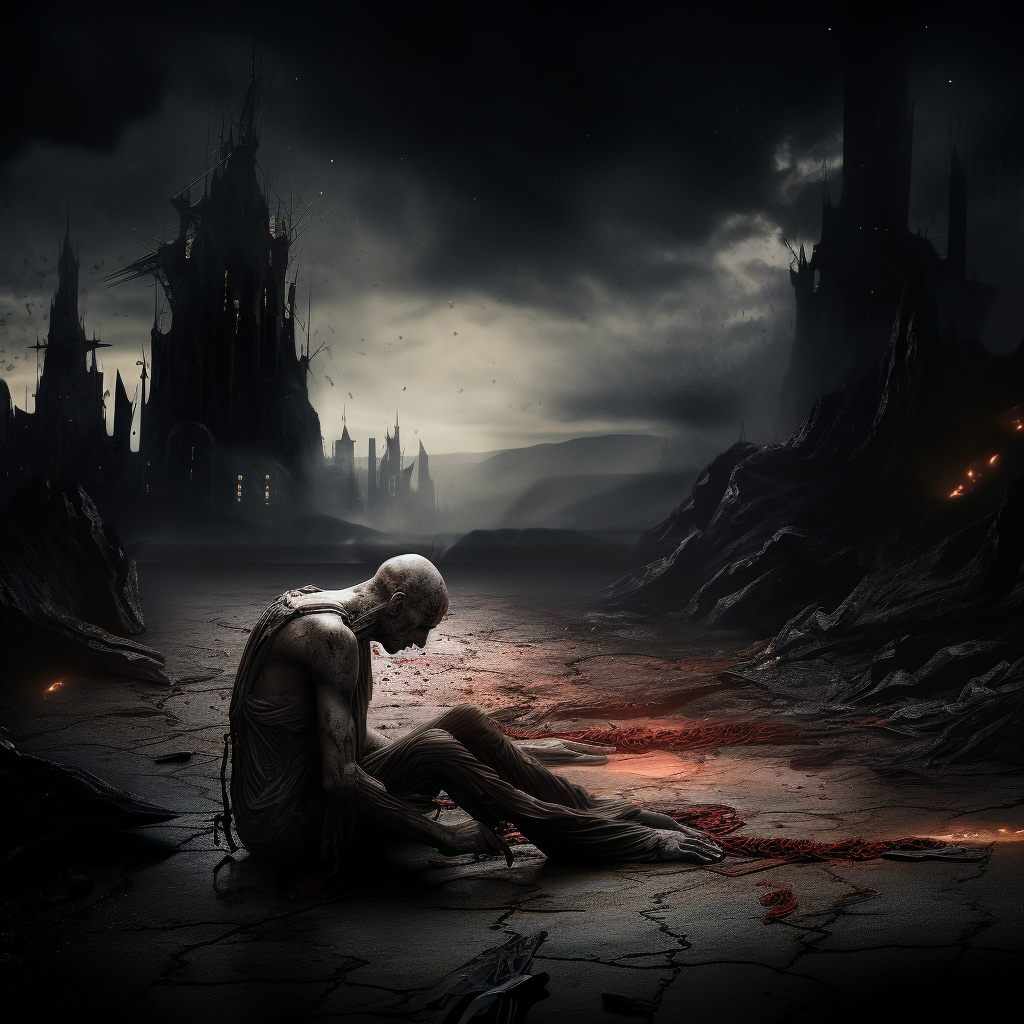
\includegraphics[width=0.3\linewidth]{a_q_s_the_human_condition_suffering_pain_evolution_618e4ef6-60ba-4d7b-a48b-e12e2a8f11cf.png}

\bigskip

In the cradle of prehistory, beneath the vast cathedral sky, \\
Ancestral whispers grapple with the howling ice-age sigh,\\
Flesh and spirit wrapped in furs, against the cold's relentless press,\\
Life a flicker in the storm, a dance with raw distress.\\

\bigskip

Fires licked the shadowed faces of those early kin,\\
Their days a spear-thrust at the dark, survival's stark discipline.\\
Each dawn bore the weight of hunger, the hunt's precarious yield,\\
Yet beneath such primal urgency, a kinship was annealed.\\

\bigskip

Leap now to the sands, where the gladiators bleed,\\
Lives unfurled as theatre, combat as a creed.\\
The roar of Rome's lust, a maddening, thunderous flood,\\
Muscle and sinew straining, arena's earth turned to mud.\\

\bigskip

Each drop of spilled lifeblood, a spectacle for the gaze,\\
Where emperors wagered with men's days,\\
Yet, in the dust and the death, a strange honor arose,\\
A brotherhood in the battle, amidst the spectacle's throes.\\

\bigskip

Move through time’s relentless march, to medieval blight,\\
Where castles loomed like omens against the candlelight.\\
Plague and torture whispered through stone corridor and street,\\
Each breath a potential thief, every heartbeat bittersweet.\\

\bigskip

But above, in their high towers, the elites draped in silk and gold,\\
Insulated from the scythe’s reach, from the suffering untold,\\
A gilded reality forked from the commoners' strife,\\
Two worlds spinning together, the double-edged sword of life.\\

\bigskip

Now we cast our eyes above, to the stars' silent song,\\
Yearning for celestial plains, for which we've yearned so long.\\
Would our touch upon new worlds spread joy or further pain?\\
Is it destiny or hubris, that through us, life's refrain?\\

\bigskip

We muse on merging with the silicon mind, our thoughts in circuit lain,\\
Would AI dream of suffering, or would its logic disdain?\\
If consciousness can be coded, what becomes of the soul?\\
Is pain mere fleshly heritage, or intelligence's toll?\\

\bigskip

In the dance of progress' shadow, where silicon sparks meet flesh,\\
Will we find newfound freedom, or entwine in suffering's mesh?\\
Is agony intrinsic, a thread through life's grand weave,\\
Or is it just a birthmark on minds that can conceive?\\

\bigskip

Suffering, the old companion, the sculptor of our kind,\\
A specter in the wilderness, in the arena, in the mind.\\
Will it be our eternal partner, as we reach for the stars,\\
A shadow stitched within us, on Earth or past Mars?\\

\bigskip

Yet, amidst the inquisition of existence, so pained, so rife,\\
Lies also the unquenchable, enduring flame of life.\\
For in each era, each struggle, against the endless night,\\
Burns the fire of human spirit, ever reaching for the light.\\

\end{center}
\end{document}

\end{center}
\end{document}
